\documentclass[11pt, spanish]{article}
\usepackage[spanish]{babel}
\selectlanguage{spanish}
\usepackage{natbib}
\usepackage{url}
\usepackage[utf8x]{inputenc}
\usepackage{graphicx}
\graphicspath{{images/}}
\usepackage{parskip}
\usepackage{fancyhdr}
\usepackage{vmargin}
\usepackage{multirow}
\usepackage{float}
\usepackage{chngpage}

\usepackage{subcaption}

\usepackage{hyperref}
\usepackage[
    type={CC},
    modifier={by-nc-sa},
    version={4.0},
]{doclicense}

\hypersetup{
    colorlinks=true,
    linkcolor=blue,
    filecolor=magenta,      
    urlcolor=cyan,
}

% para codigo
\usepackage{listings}
\usepackage{xcolor}



%% configuración de listings

\definecolor{listing-background}{HTML}{F7F7F7}
\definecolor{listing-rule}{HTML}{B3B2B3}
\definecolor{listing-numbers}{HTML}{B3B2B3}
\definecolor{listing-text-color}{HTML}{000000}
\definecolor{listing-keyword}{HTML}{435489}
\definecolor{listing-identifier}{HTML}{435489}
\definecolor{listing-string}{HTML}{00999A}
\definecolor{listing-comment}{HTML}{8E8E8E}
\definecolor{listing-javadoc-comment}{HTML}{006CA9}

\lstdefinestyle{eisvogel_listing_style}{
  language         = c++,
%$if(listings-disable-line-numbers)$
%  xleftmargin      = 0.6em,
%  framexleftmargin = 0.4em,
%$else$
  numbers          = left,
  xleftmargin      = 0em,
 framexleftmargin = 0em,
%$endif$
  backgroundcolor  = \color{listing-background},
  basicstyle       = \color{listing-text-color}\small\ttfamily{}\linespread{1.15}, % print whole listing small
  breaklines       = true,
  frame            = single,
  framesep         = 0.19em,
  rulecolor        = \color{listing-rule},
  frameround       = ffff,
  tabsize          = 4,
  numberstyle      = \color{listing-numbers},
  aboveskip        = 1.0em,
  belowskip        = 0.1em,
  abovecaptionskip = 0em,
  belowcaptionskip = 1.0em,
  keywordstyle     = \color{listing-keyword}\bfseries,
  classoffset      = 0,
  sensitive        = true,
  identifierstyle  = \color{listing-identifier},
  commentstyle     = \color{listing-comment},
  morecomment      = [s][\color{listing-javadoc-comment}]{/**}{*/},
  stringstyle      = \color{listing-string},
  showstringspaces = false,
  escapeinside     = {/*@}{@*/}, % Allow LaTeX inside these special comments
  literate         =
  {á}{{\'a}}1 {é}{{\'e}}1 {í}{{\'i}}1 {ó}{{\'o}}1 {ú}{{\'u}}1
  {Á}{{\'A}}1 {É}{{\'E}}1 {Í}{{\'I}}1 {Ó}{{\'O}}1 {Ú}{{\'U}}1
  {à}{{\`a}}1 {è}{{\'e}}1 {ì}{{\`i}}1 {ò}{{\`o}}1 {ù}{{\`u}}1
  {À}{{\`A}}1 {È}{{\'E}}1 {Ì}{{\`I}}1 {Ò}{{\`O}}1 {Ù}{{\`U}}1
  {ä}{{\"a}}1 {ë}{{\"e}}1 {ï}{{\"i}}1 {ö}{{\"o}}1 {ü}{{\"u}}1
  {Ä}{{\"A}}1 {Ë}{{\"E}}1 {Ï}{{\"I}}1 {Ö}{{\"O}}1 {Ü}{{\"U}}1
  {â}{{\^a}}1 {ê}{{\^e}}1 {î}{{\^i}}1 {ô}{{\^o}}1 {û}{{\^u}}1
  {Â}{{\^A}}1 {Ê}{{\^E}}1 {Î}{{\^I}}1 {Ô}{{\^O}}1 {Û}{{\^U}}1
  {œ}{{\oe}}1 {Œ}{{\OE}}1 {æ}{{\ae}}1 {Æ}{{\AE}}1 {ß}{{\ss}}1
  {ç}{{\c c}}1 {Ç}{{\c C}}1 {ø}{{\o}}1 {å}{{\r a}}1 {Å}{{\r A}}1
  {€}{{\EUR}}1 {£}{{\pounds}}1 {«}{{\guillemotleft}}1
  {»}{{\guillemotright}}1 {ñ}{{\~n}}1 {Ñ}{{\~N}}1 {¿}{{?`}}1
  {…}{{\ldots}}1 {≥}{{>=}}1 {≤}{{<=}}1 {„}{{\glqq}}1 {“}{{\grqq}}1
  {”}{{''}}1
}
\lstset{style=eisvogel_listing_style}


\usepackage[default]{sourcesanspro}

\setmarginsrb{2 cm}{1 cm}{2 cm}{2 cm}{1 cm}{1.5 cm}{1 cm}{1.5 cm}

\title{Práctica 2:\\
Satisfacción de restricciones  \hspace{0.05cm} }                           
\author{Antonio David Villegas Yeguas}                             
\date{\today}                                           


\makeatletter
\let\thetitle\@title
\let\theauthor\@author
\let\thedate\@date
\makeatother

\pagestyle{fancy}
\fancyhf{}
\rhead{\theauthor}
\lhead{\thetitle}
\cfoot{\thepage}

\begin{document}

%%%%%%%%%%%%%%%%%%%%%%%%%%%%%%%%%%%%%%%%%%%%%%%%%%%%%%%%%%%%%%%%%%%%%%%%%%%%%%%%%%%%%%%%%

\begin{titlepage}
    \centering
    \vspace*{0.3 cm}
    
\includegraphics[scale = 0.50]{ugr.png}\\[0.7 cm]
    %\textsc{\LARGE Universidad de Granada}\\[2.0 cm]   
    \textsc{\large 3º CSI 2019/20 - Grupo 1}\\[0.5 cm]            
    \textsc{\large Grado en Ingeniería Informática}\\[0.5 cm]              
    \rule{\linewidth}{0.2 mm} \\[0.2 cm]
    { \huge \bfseries \thetitle}\\
    \rule{\linewidth}{0.2 mm} \\[1 cm]
    
    \begin{minipage}{0.4\textwidth}
        \begin{flushleft} \large
            \emph{Autor:}\\
            \theauthor\\ 
			 \emph{DNI:}\\
            77021623-M
            \end{flushleft}
            \end{minipage}~
            \begin{minipage}{0.4\textwidth}
            \begin{flushright} \large
            \emph{Asignatura: \\
            Técnicas de los Sistemas Inteligentes}   \\     
            \emph{Correo:}\\
            advy99@correo.ugr.es           
        \end{flushright}
    \end{minipage}\\[0.5cm]
  
    {\large \thedate}\\[0.5cm]
    %{\url{https://github.com/advy99/TSI/}}
    {\doclicenseThis}
 	
    \vfill
    
\end{titlepage}

%%%%%%%%%%%%%%%%%%%%%%%%%%%%%%%%%%%%%%%%%%%%%%%%%%%%%%%%%%%%%%%%%%%%%%%%%%%%%%%%%%%%%%%%%

%\tableofcontents
%\pagebreak

%%%%%%%%%%%%%%%%%%%%%%%%%%%%%%%%%%%%%%%%%%%%%%%%%%%%%%%%%%%%%%%%%%%%%%%%%%%%%%%%%%%%%%%%%

\section*{Introducción}

En esta práctica se nos propone resolver distintos problemas de satisfacción de restricciones. En cada problema, dado su enunciado, hay que decidir cuales son las variables que intervienen en el problema, el dominio que tienen dichas variables, y que restricciones tienen esas variables, como bien sabemos tras estudiar el tema 2 de la teoría de la asignatura.

Para resolver estos problemas propuestos usaremos la herramienta MiniZinc, un lenguaje de modelado de restricciones que cuenta con un IDE con el que podremos representar los problemas y resolverlos. Este lenguaje cuenta con distintas herramientas para resolver los problemas de satisfacción de restricciones (\textit{CSP solvers}), aunque para esta práctica solo utilizaremos Gecode, instalado por defecto.

\section{Ejercicio 1}

Puzzle Cripto-aritmético. El siguiente problema plantea un problema criptoaritmético, de forma que cada letra codifica un único dígito (es decir, un número entero en [0,9]) y cada dígito está asignado a una única letra. Se pide encontrar una asignación de dígitos a letras que satisfaga la siguiente suma:

\begin{lstlisting}
     TESTE
 +   FESTE
 +   DEINE
  =========
    KRAFTE
\end{lstlisting}

\subsection{Variables}

Tendremos 10 variables, una por letra. En MiniZinc lo representaremos con un array de 10 posiciones.

\subsection{Dominio de las variables}

Cada variable es un entero entre el número 0 y el 9 (ambos incluidos).

Usaremos variables auxiliares para gestionar los acarreos.

\subsection{Restricciones}

\textbf{1:} Cada variable tiene que tomar un valor distinto. Esto lo conseguiremos con el uso de la función \texttt{alldifferent(array)} de MiniZinc.

\textbf{2:} La suma de cada columna tiene que coincidir (con su respectivo acarreo). Usaremos 5 variables para almacenar el acarreo de cada suma, y haremos uso de \texttt{constraint} para hacer que las sumas sumando el acarreo (y dividido por 10, para que el resultado este entre 0..9) sean igual a la letra correspondiente. El acarreo será la misma operación, pero aplicando la operación módulo 10.


\subsection{Resultado}

\begin{figure}[H]
  \centering
      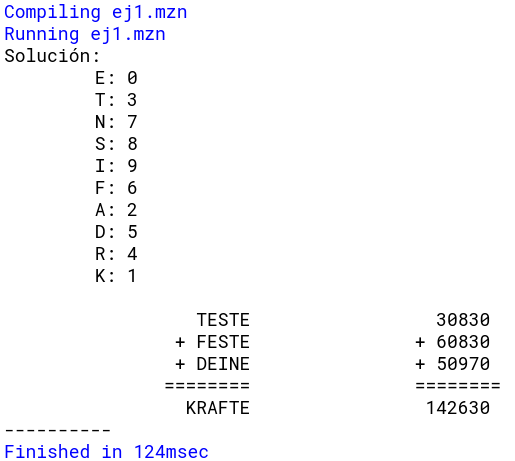
\includegraphics[scale = 0.30]{sol1.png}
 		 \caption{Solución obtenida para el ejercicio 1.}
  		\label{fig:ej1}

\end{figure}

\section{Ejercicio 2}
Encontrar un número X de 10 dígitos que satisfaga que el primer dígito de X representa el número de 0s en X, el segundo dígito de X representa el número de 1s en X, etc...

Por ejemplo, el número X=6210001000 satisface dicha condición.

\subsection{Variables}

Usaremos un array con 10 posiciones, de la 0 a la 9 (ambos incluidos) para representar el número X.

\subsection{Dominio de las variables}

Las variables son números enteros de 0 a 9.

\subsection{Restricciones}

El indice del dígito equivale al número de veces que aparece el dígito en el número X. Esto lo conseguimos en MiniZinc con un bucle, en el que para todo i desde 0 hasta 9, tiene que aparecer i veces.

\subsection{Resultado}

\begin{figure}[H]
  \centering
      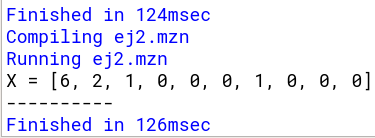
\includegraphics[scale = 0.50]{sol2.png}
 		 \caption{Solución obtenida para el ejercicio 2.}
  		\label{fig:ej2}

\end{figure}


\section{Ejercicio 3}

Encontrar una asignación de horarios que satisfaga las siguientes condiciones (condiciones en la sección de restricciones).

\subsection{Variables}

Usaremos un array con tantos elementos como profesores.

También usaremos una matriz con tantas filas como profesores y dos columnas, para representar el inicio y fin del horario de cada profesor.

\subsection{Dominio de las variables}

El array para la asignación de profesores puede tomar valores entre 9 y 14, las horas donde puede comenzar una clase, es decir, si, por ejemplo, toma el valor 9 en la posición 2, quiere decir que el profesor 2 da clase de 9:00 a 10:00.

La matriz puede tomar valores entre 9 y 15, el horario dado.

\subsection{Restricciones}

Las restricciones son que un aula solo puede estar ocupada por un profesor, esto lo hemos conseguido al usar una array con una posición por hora.

Otra restricción a tener en cuenta es que las clases son de 1 hora, luego no se repiten ningún profesor, usaremos \texttt{alldifferent(profesores)} para tener en cuenta esta restricción.

Cada profesor tiene un horario disponible. Esto lo solucionamos haciendo uso de la matriz de horarios, asegurando que la posición de un profesor en el array es mayor o igual que la hora de inicio y menor que la hora de fin (en la hora de fin menor estricto, ya que si un horario va de 9:00 a 13:00, no se puede dar clase a las 13:00 - 14:00).

\subsection{Resultado}


\begin{figure}[H]
  \centering
      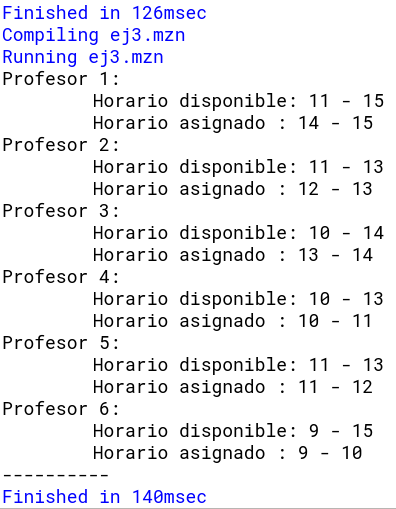
\includegraphics[scale = 0.30]{sol3.png}
 		 \caption{Solución obtenida para el ejercicio 3.}
  		\label{fig:ej3}

\end{figure}

\section{Ejercicio 4}
Encontrar una asignación de horarios que satisfaga las siguientes condiciones (condiciones en las restricciones).

\subsection{Variables}

Usaré una matriz de asignaciones, con tantas filas como aulas, y tantas columnas como horas permitidas.

Usaré variables auxiliares para referirme a las asignaturas de forma más cómoda.

\subsection{Dominio de las variables}

La matriz de asignaciones ira de 0 hasta 12, 0 es un hueco libre, y de 1 a 12 un número por asignatura. Las asignaturas 1, 2 y 3 representarán IA, TSI y FBD respectivamente del grupo 1, las asignaturas 4, 5 y 6 las del grupo 2, etc.

\subsection{Restricciones}

En una misma franja horaria, lo que se imparte en las distintas clases ha de ser distinto. Esto lo conseguiremos en MiniZinc haciendo un bucle en el que para todas las horas i, la clase de las distintas aulas j sea distinta.

También tenemos que asegurarnos que si en una hora en un aula se da una clase del grupo 1 (por ejemplo), en las demás aulas no puede haber clases del mismo grupo. Esto lo haremos para todos los grupos.

Esto último también lo tenemos que hacer para las asignaturas que imparten los profesores, por ejemplo, si a una hora se imparte IA2, no se puede impartir TSI1 ya que las imparte el mismo profesor.

También contamos con las restricciones de que el profesor 2 no puede dar clase a las 10:00 y el profesor 4 no puede dar clase a las 9:00. Simplemente hacemos que para todas las aulas, en esa franja horaria no esté ninguna asignatura impartida por dichos profesores.

Por último, comprobamos que cada asignatura aparece una sola vez.

\subsection{Resultado}


\begin{figure}[H]
  \centering
      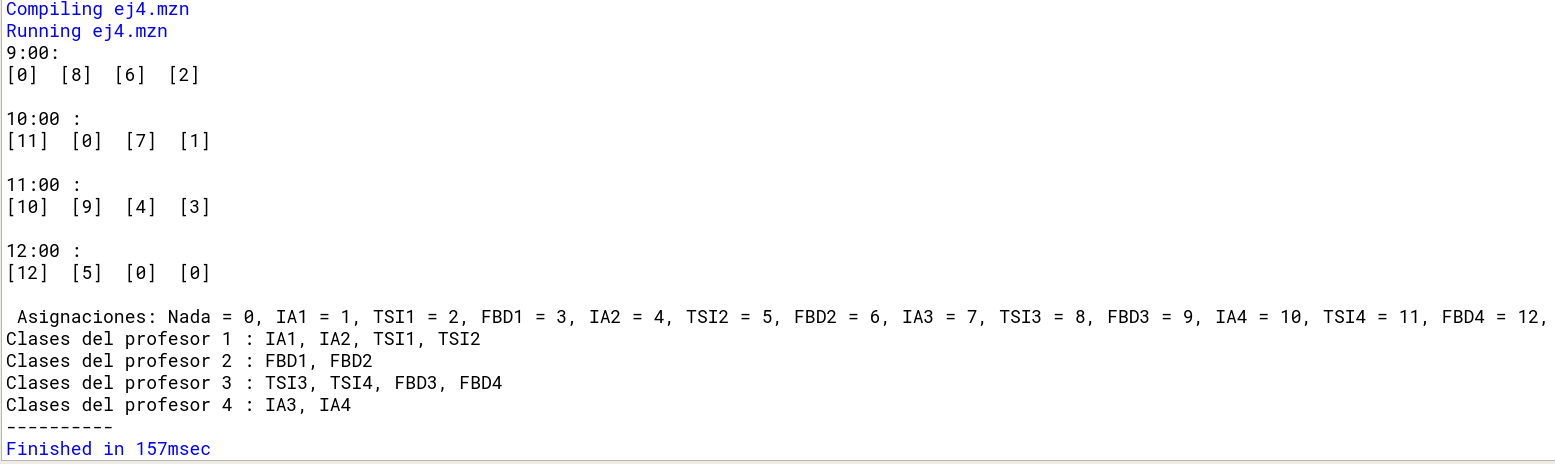
\includegraphics[scale = 0.30]{sol4.png}
 		 \caption{Solución obtenida para el ejercicio 4.}
  		\label{fig:ej4}

\end{figure}


\section{Ejercicio 5}

Encontrar una asignación de horarios que satisfaga las siguientes condiciones.

\subsection{Variables}

Hora de inicio y hora de fin. La hora de fin serán 5 horas después de la hora de inicio, para tener esas 6 horas que comenta el ejercicio. Eliminar el valor por defecto para que pregunte la hora de inicio al usuario.

Un array por cada día de la semana.

Un array con las horas necesarias de cada asignatura.

\subsection{Dominio de las variables}

La hora de inicio y hora de fin son enteros.

Los distintos arrays representando los días de la semana almacenarán valores de 0 a 9, donde 0 es que no se asigna asignatura y del 1 al 9 las distintas asignaturas.

El array de horas necesarias toma valores de 1 a 4, que son el número de horas dadas. Podría usarse como int al estar fijo al inicio del programa.

\subsection{Restricciones}

Cada asignatura aparece en todos los días exactamente el número de horas necesarias almacenado en el array de horas necesarias.

Las asignaturas 1, 3, 4, 5 y 8 se impartirán en bloques de dos horas, y las demás en bloques de una hora, además solo se puede dar un bloque por día de la semana. Esto lo conseguiremos haciendo que las apariciones de una asignatura un día solo puede ser igual a  0 (no se imparte ese día) o 1 o 2 (dependiendo del tamaño del bloque).

Los bloques se imparten en horas consecutivas, luego nos aseguraremos que si en una posición i aparece una asignatura de dos horas, en una de las posiciones contiguas también aparece la asignatura.

Se pide que la cuarta hora se deje libre para el recreo, luego todos los días, la hora correspondiente a la hora de comienzo más tres (el comienzo de la cuarta franja horaria) tendrá el valor 0.

También tenemos que tener en cuenta que si un bloque aparece un día, no puede aparecer más bloques impartidos por el mismo profesor, a excepción del profesor 4. Esto lo conseguiremos asegurando que si un día aparece una asignatura impartida por un profesor, esta solo aparece el número de horas correspondiente a un bloque y no aparecen otras asignaturas impartidas por el profesor.

\subsection{Resultado}


\begin{figure}[H]
  \centering
      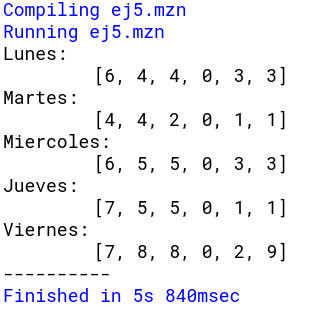
\includegraphics[scale = 0.40]{sol5.png}
 		 \caption{Solución obtenida para el ejercicio 5.}
  		\label{fig:ej5}

\end{figure}

Comentar que mientras en otros ejercicios el tiempo de ejecución es inapreciable, en este ejercicio no ocurre debido a la complejidad de las restricciones, y vemos como tenemos que esperar unos pocos segundos par obtener la solución.


\newpage

\section{Ejercicio 6}
Cinco personas de cinco regiones diferentes viven en las primeras cinco casas contiguas de una calle. Practican cinco profesiones distintas, y cada uno tiene un animal y una bebida favoritos, todos ello diferentes. Las casas están pintadas con diferentes colores. Ademas sabemos lo siguiente (restricciones en el PDF, más adelante explicaré algunas).

Resolver el problema de forma que podamos responder: ¿dónde está la cebra y quién bebe agua?

\subsection{Variables}

Cinco vectores con 5 posiciones, cada no representará la asignación que haremos de nacionalidades, color de casa, máscotas, bebidas y profesiones.

Variables auxiliares que usaremos para cumplir las restricciones.

\subsection{Dominio de las variables}

Todos los vectores tendrán un enumerado asociado, en el que están sus posibles valores, por ejemplo usaremos un enumerado de colores, donde estarán los valores rojo, amarillo, azul, verde y blanco.

\subsection{Restricciones}

Como restricciones tenemos la lista dada en el enunciado. Diferenciamos dos restricciones, en las que interviene un único array, por ejemplo que el andaluz vive en la casa de la izquierda, que se resolverá haciendo que la primera posición del array de nacionalidades tenga el valor andaluz, o el segundo tipo, donde intervienen dos arrays, por ejemplo el vasco vive en la casa roja, lo que haremos es hacer que el indice de la casa roja sea el mismo que el indice del array donde está el valor vasco en el array de nacionalidades.

\subsection{Resultado}


\begin{figure}[H]
  \centering
      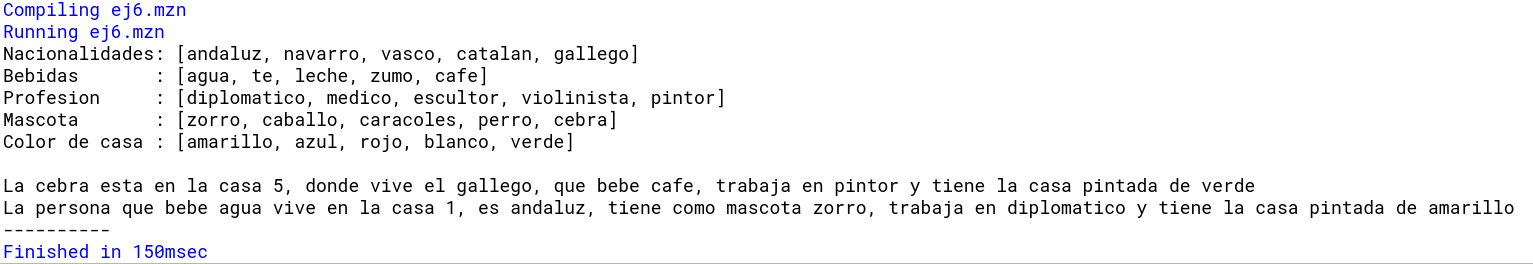
\includegraphics[scale = 0.30]{sol6.png}
 		 \caption{Solución obtenida para el ejercicio 6.}
  		\label{fig:ej6}

\end{figure}

\newpage

\section{Ejercicio 7}

En la tabla adjunta aparece la información necesaria para llevar a cabo la construcción de una casa. En la primera columna aparecen los indentificadores de las tareas necesarias para
construirla. En la segunda columna aparece la descripción de cada una de estas. En la tercera columna se muestra la duración (en días) de cada una de las tareas. Y la cuarta columna muestra la relación de precedencia entre tareas: por ejemplo, si el contenido de la celda correspondiente a la tarea “F” es “C,D" se debe interpretar como que “las tareas C y D deben finalizarse antes que comience la tarea “F”. Se pide encontrar una asignación de tiempos de inicio a estas tareas de forma que se pueda construir la casa en el menor tiempo posible, asumiendo que cada tarea la realiza un único trabajador y que se disponen de tantos trabajadores como se necesiten.

\subsection{Variables}

Array de nueve elementos con al duración de cada tarea.

Coste de la solución.

Matriz de predecesoras. La usaremos para almacenar las tareas que tienen que ser realizadas antes que otras.

Array de con las predecesoras ordenadas.

Array con la asignación final que mostraremos como solución.

\subsection{Dominio de las variables}

La matriz de predecesoras y el array de predecesoras van desde 0 hasta el número de tareas menos 1, 0 representa que no tiene predecesora. Es una matriz con dos columnas para representar las tareas que tienen varias predecesoras.

El coste de la solución tiene dominio en los enteros.

Los distintos arrays tienen dominio entre 1 y 9, el número de tareas, menos el de predecesoras ordenadas, que también incluye el 0 al tener tareas sin predecesoras.

\subsection{Restricciones}

Las restricciones es que se de el orden en el que se tienen que hacer las tareas, esto lo haremos con el array de predecesoras ordenadas, lo recorreremos y si un elemento coincide con el de predecesoras, sabemos que esa tarea se tiene que realizar antes, por lo que en el array solución tendrá el mismo valor. Esto también hace que por ejemplo, si varias tareas se realizan en paralelo, podamos pasar del indice 2 al 5, porque la segunda, tercera y cuarta tarea se ejecutan en paralelo.

Otra restricción es que el coste sea mínimo, para esto usaremos la opción de MiniZinc \texttt{solve minimize coste}. Para obtener el coste de una tarea he declarado una función recursiva en MiniZinc, de forma que si la tarea dada tiene como predecesoras el 0, devuelve el coste de esa tarea, y si no el máximo del coste de las dos predecesoras más el coste de la propia tarea.

El coste por tanto será la llamada a esta función con la última tarea del array de predecesoras ordenadas más uno (el array de predecesoras va de 0 a 8 y las tareas de 0 a 9).

\subsection{Resultado}


\begin{figure}[H]
  \centering
      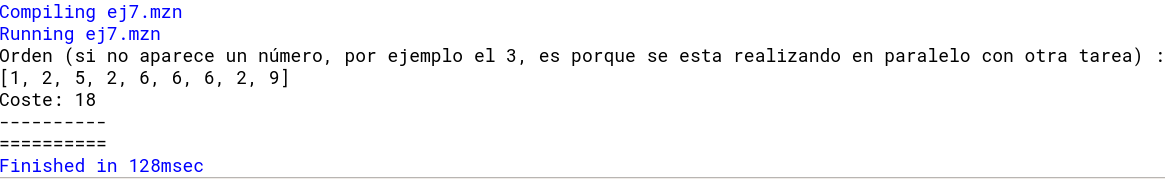
\includegraphics[scale = 0.30]{sol7.png}
 		 \caption{Solución obtenida para el ejercicio 7.}
  		\label{fig:ej7}

\end{figure}


%\section{Ejercicio 8}

%\subsection{Variables}

%\subsection{Dominio de las variables}

%\subsection{Restricciones}

%\subsection{Resultado}


%\section{Ejercicio 9}

%\subsection{Variables}

%\subsection{Dominio de las variables}

%\subsection{Restricciones}

%\subsection{Resultado}


\section{Ejercicio 10}

Un turista desea llenar su mochila con varios objetos para hacer un viaje. El peso máximo que aguanta la mochila son 275kg, y cada objeto tiene distinto grado de preferencia para el turista (la preferencia se mide en una escala de 0 a 200, donde los números más altos representan los objetos más deseados por el turista). En la tabla siguiente se muestran los objetos, su peso y su preferencia. Encontrar el conjunto de objetos cuya suma de preferencias sea máxima sin exceder el peso máximo que aguanta la mochila.



\subsection{Variables}

Array de longitud 12 (ya que son 12 objetos) de los distintos pesos de los objetos.

Array de longitud 12 (ya que son 12 objetos) de las preferencias de los distintos objetos.

Array de longitud 12 (ya que son 12 objetos) de objetos seleccionados.

Peso máximo.

Peso en la mochila.

Preferencia de los objetos introducidos en la mochila.

\subsection{Dominio de las variables}

El array de pesos, el de preferencias, y las variables usadas son de tipo int, al poder contener enteros que en principio no están limitados.

El array de objetos seleccionados es un array de elementos tipo bool, en el que una posición i = false representa que el objeto i no se ha seleccionado y true representa que si se ha seleccionado.

\subsection{Restricciones}

Las restricciones son que la suma de los objetos seleccionados (marcados como true en el array de objetos seleccionados) sea menor que el tamaño máximo (275 en el ejercicio).

Otra restricción es que la preferencia de los objetos seleccionados sea máxima. Esto lo haremos sumando la preferencia de los objetos marcados a true, y usando la opción \texttt{solve maximize preferencia}, en el que MiniZinc lo resolverá intentando que el valor de esa variable sea el más alto posible.

\subsection{Resultado}

\begin{figure}[H]
  \centering
      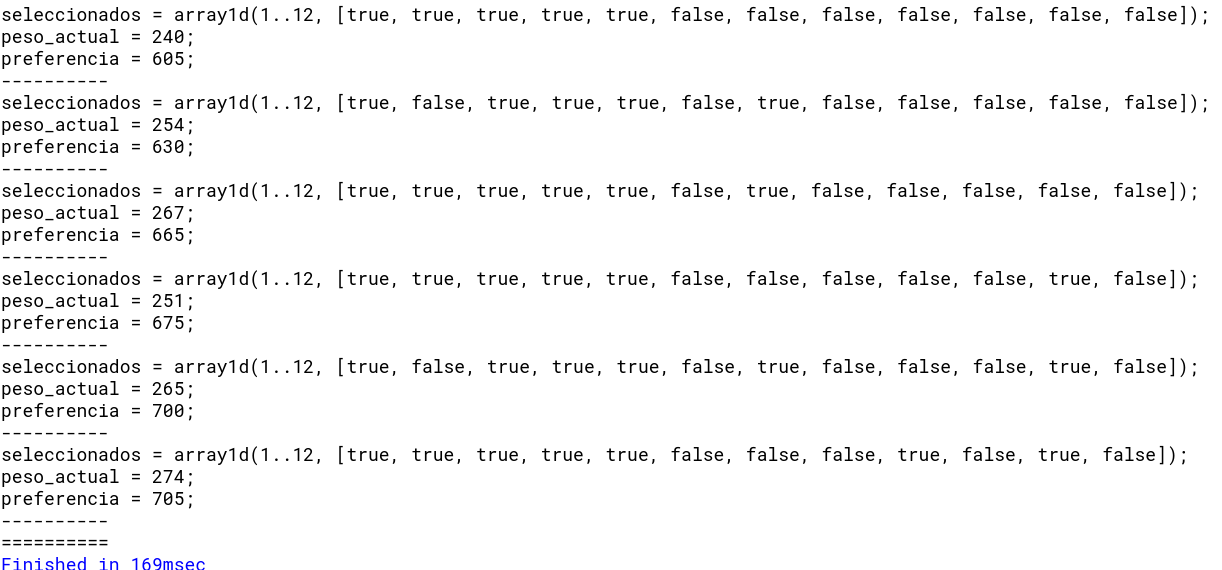
\includegraphics[scale = 0.30]{sol10.png}
 		 \caption{Solución obtenida para el ejercicio 10.}
  		\label{fig:ej10}

\end{figure}

En este caso, al usar maximize, MiniZinc nos muestra por que situaciones ha ido pasando antes de encontrar la solución.

\end{document}
